
We first plot the function $f_1$ to have an intuition. 

\begin{center}
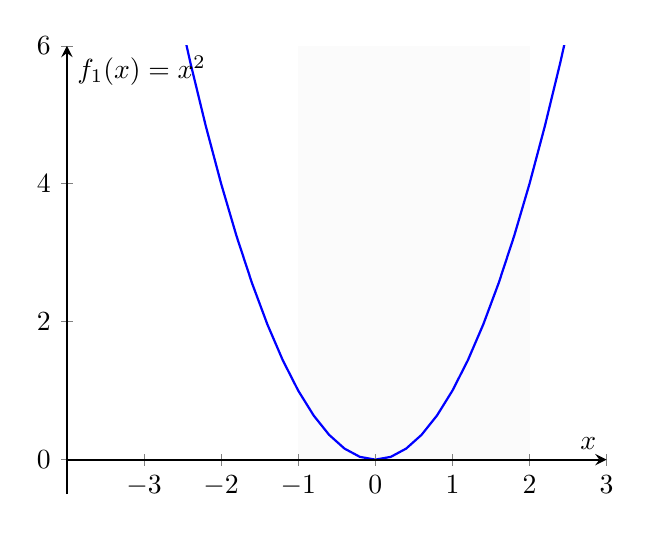
\begin{tikzpicture}
\begin{axis}[ xlabel={$x$}, ylabel={$f_1(x)=x^2$}
,axis on top=true
,axis lines=middle
,samples=41, thick
,domain=-4:4, xmin=-4, xmax=3,
    ymin=-0.5, ymax=6,
    axis y line = left
  ]

\fill[fill=gray!15,fill opacity=0.2,draw=none] (-1,0) rectangle (2,6);  
\addplot+ [no marks] {x^2};
\end{axis}
\end{tikzpicture}
\end{center}

The infimum of  $x^2$ on $\R$ is 0:
\[
\inf_{x \in \R} x^2 = 0.
\]
Indeed, for each $M > 0$, there exists 
\[
y = \frac{\sqrt{M}}{2}
\]
such that $y^2 = \frac{M}{4} < M$.
The function has also a minimum at $x^*=0$, as
\[
f_1(x^*) = \inf_{x \in \R} x^2 = 0.
\]

When the constraints are introduced, the same arguments can be used to
reach the same conclusions: the infimum is 0, and $x^*=0$ is an optimum.




We now analyze the function $f_2$.


\begin{center}
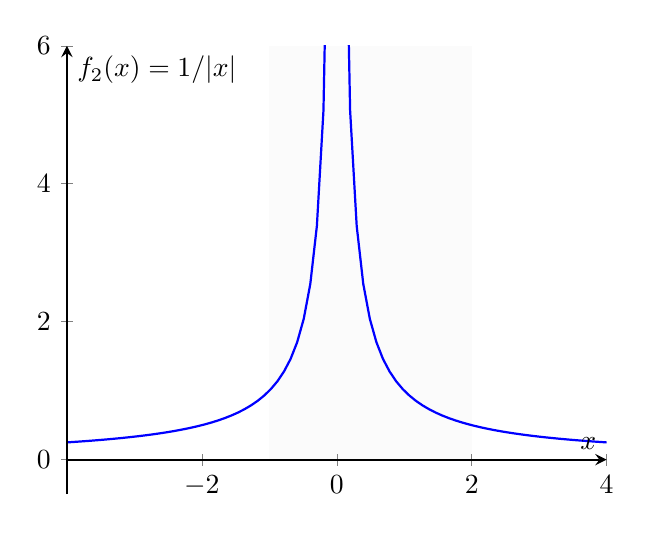
\begin{tikzpicture}
\begin{axis}[ xlabel={$x$}, ylabel={$f_2(x)=1/|x|$}
,axis on top=true
,axis lines=middle
,samples=41, thick
, xmin=-4, xmax=4,
    ymin=-0.5, ymax=6,
    axis y line = left
]
\fill[fill=gray!15,fill opacity=0.2,draw=none] (-1,0) rectangle (2,6) ;
\addplot+ [domain=-4:-0.1,no marks,blue,]  {1/abs(x)};
\addplot+ [domain=0.1:4,no marks,blue]  {1/abs(x)};
\end{axis}
\end{tikzpicture}
\end{center}


The infimum of $1/|x|$ on $\R$ is $0$:
\[
\inf_{x \in \R} \frac{1}{|x|} = 0.
\]
Indeed, for each $M>0$, there exists 
\[
y = \frac{2}{M}
\]
such that $f_2(y) = \frac{M}{2} < M$.
However, there is no minimum, as there is no $x$ such that
\[
\frac{1}{|x|} = 0.
\]

The infimum of $1/|x|$ on $Y=\{x \in \R|-1\leq x \leq 2\}$ is $0.5$.
Indeed, for each $M>0.5$, there exists 
\[
y = 2 \in Y
\]
such that $f_2(y) = 0.5 < M$.
And the minimum is $x^*=2$, as
\[
f_2(x^*)=0.5 = \inf_{x \in Y} \frac{1}{|x|}.
\]


Finally, we analyze the function $f_3$.


\begin{center}
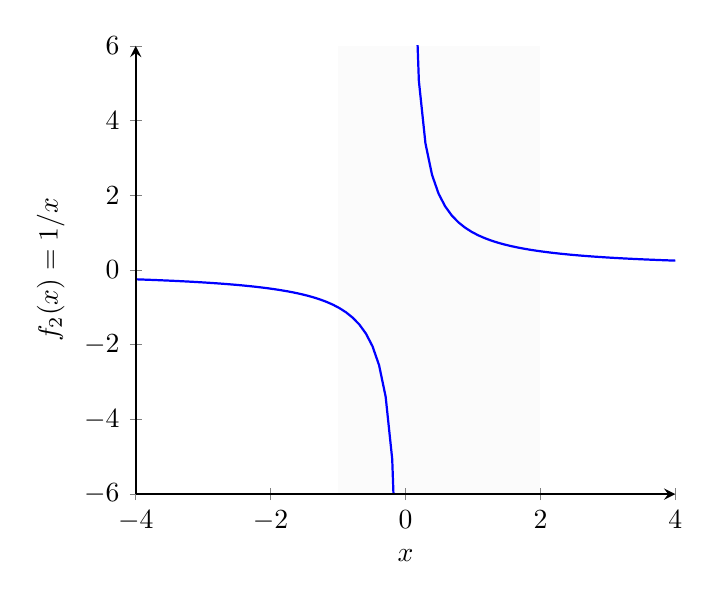
\begin{tikzpicture}
\begin{axis}[ xlabel={$x$}, ylabel={$f_2(x)=1/x$}
,axis on top=true
,axis x line=bottom
,samples=41, thick
, xmin=-4, xmax=4,
    ymin=-6, ymax=6,
    axis y line = left
]
\fill[fill=gray!15,fill opacity=0.2,draw=none] (-1,-6) rectangle (2,6) ;
\addplot+ [domain=-4:-0.1,no marks,blue,]  {1/x};
\addplot+ [domain=0.1:4,no marks,blue]  {1/x};
\end{axis}
\end{tikzpicture}
\end{center}

There is no infimum on $\R$. Indeed, the function is not bounded from
below. As the infimum is the best lower bound, and there is no lower
bound, there is no infimum. Consequently, there is no optimum
either. As the function is also not bounded from below on the interval
$[-1:2]$, we reach the same conclusions for the constrained case. 

